\section{Administrative Interface}
% - admin web server
% uses httprequesthandlers
% velocity templates
% based off phpBB admin interface
% has a few basic functions, and allows admins to administer those
% view connected clients
% update configuration values
% upload images
% execute specific commands
% perform backup
% restore backups
One of the last components to be added was the administrative interface. Calico now had a headless server, and we needed a way to remotely manage it. We decided against building the interface within the Calico client - we wanted to keep the client as lightweight as possible. 
We decided to create an easy to use web-based interface that would allow the Calico server to be managed easily using a web browser.

The administrative interface only provided basic management abilities. The core abilities it provided were:
\begin{itemize}\itemsep1pt

\item
\textbf{Easily modify settings}.
We needed the ability to modify the settings of an existing Calico instance easily. What was created was a page that listed all the configuration variables and easily let the administrator modify those values. When saved, the Calico server could then be restarted if needed to reflect the configuration changes.

\item
\textbf{View currently connected clients}. 
This was helpful in the classroom environment to be able to see all users who were currently connected to the server. In the future we planned to add the ability to ``kick'' clients from the server, but this was never full developed.

\item
\textbf{Perform backups and restoration of sessions}.
One of the major requirements was the ability to easily generate a backup of an entire session. Our goal was to provide an easily way to download a backup file that represented the current state of the server. It needed to contain all the data required to fully restore all canvases and any scraps, strokes, or arrows that may be contained in the canvas. Once we created the backup system, we needed a way for a server to restore any backup. Our administrative interface provided an easy to use form where a backup file could be selected and then uploaded directly to a running server. The server would then read the contents of this file and import all data into the server. Restoring a backup essentially wiped any existing content and recreated the entire session from scratch. Once a restoration had been performed, clients could reconnect and they would see all the data, just as it was when the backup was created.

\end{itemize}

These few requirements were the driving force behind the administrative interface. It stands as a very barebones and minimalistic interface that provides functions that we decided were essential to operation. This administrative interface has proved invaluable when generating and restoring backups. Having a backup of sessions provides users with a greater level of reassurance that any work they have made will not be lost should anything happen to the server.

% list of website paths and each one is mapped to a request handler for that specific action
% 
To keep the admin system lightweight, we decided to utilize the \texttt{HttpComponents} library provided by the Apache Foundation\cite{apache:http}. This library provides a single webserver endpoint that will route all web requests to a predefined list of request handler endpoints. These endpoints are specified in the \texttt{AdminRequestListenerThread} class within Calico. The most important part of this request handler is the ``request registry''. This registry acts as a routing engine that will route requests made to certain endpoints to a specific request handler designed to handle that request.

\begin{figure}[htb]
  \centering
  \small
  \verbatiminput{figures/java/request_registry.java}
  \normalsize
  \caption{Administration interface routing example}
  \label{code:request_registry}
\end{figure}

In figure \ref{code:request_registry}, you can see a code snippet of the routing table. The important part is the call to \texttt{reqistry.register}. In this snippet, you can see that any requests that are sent to \texttt{/gui/config/} will be sent to the \texttt{ConfigIndexRH} class to be processed. This allowed us to break the administration system into logical components each designed to handle a different aspect of the server. 

\begin{figure}[htb]
  \centering
  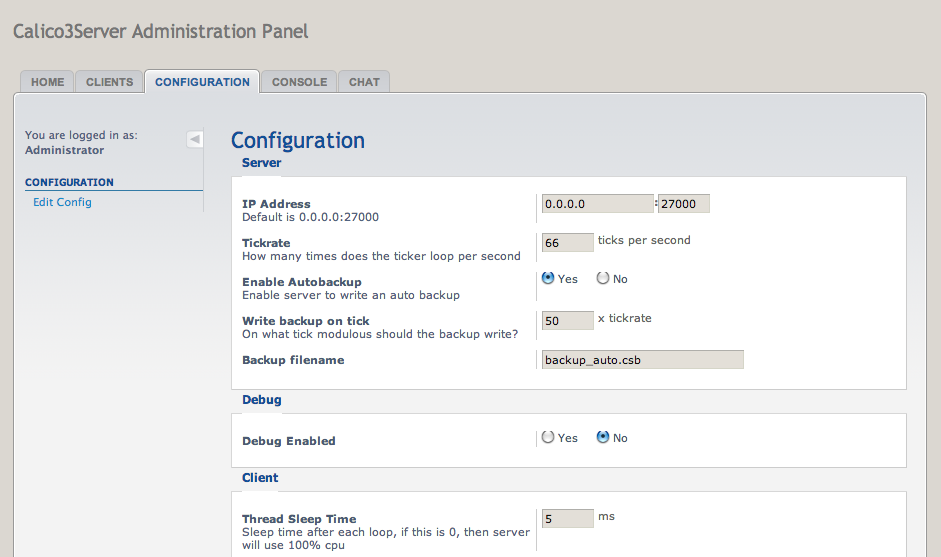
\includegraphics[width=0.8\textwidth]{admin_ui.png}
  \caption{Admin configuration form (/gui/config/)}
  \label{fig:admin_config}
\end{figure}

One example request handler would be the \texttt{ConfigIndexRH} class that was mentioned above. This class was responsible for two separate tasks. The first task was to process a \texttt{GET} request to \texttt{/gui/config/} which meant that the configuration form should be displayed in the user's browser (an example form can be seen in figure \ref{fig:admin_config}). To easily create the HTML required for the administration interface, we decided to use a templating framework that would allow us easily write HTML that contained placeholders that could be rendered by the request handlers. The template framework that we chose to use was Apache's Velocity\cite{velocity} framework. We decided to use Velocity because of its ease-of-use as well as its powerful language that allowed us to create various macros to easily abstract common interface elements. The interface look-and-feel was copied from the administrative interface of an open-source forum system known as PhpBB\cite{phpbb}. Figure \ref{code:tpl_config} shows a snippet of the template language that was used to generate the configuration form seen in figure \ref{fig:admin_config}.

\begin{figure}[htb]
  \centering
  \small
  \verbatiminput{figures/tpl/config.tpl}
  \normalsize
  \caption{Snippet of the Velocity template for configuration page}
  \label{code:tpl_config}
\end{figure}

The second task of the configuration request handler was to process a \texttt{POST} request to the same endpoint. This request was for a form submission, which instructed the server to update the configuration settings on the server to reflect the values entered in the configuration form.